% python classes slides - profiling and optimization
% (c) 2014 Kostiantyn Danylov aka koder 
% koder.mail@gmail.com
% distributed under CC-BY licence
% http://creativecommons.org/licenses/by/3.0/deed.en

\documentclass{article}
% XeLaTeX
\usepackage{xltxtra}
\usepackage{xunicode}
\usepackage{listings}
\usepackage[landscape]{geometry}

% Fonts
\setmainfont{DejaVu Sans} %{Arial}
\newfontfamily\cyrillicfont{Nimbus Roman No9 L} %{Arial}
\setmonofont{Courier New}
%\setmonofont{Ubuntu Mono}

%\setmonofont{DejaVu Sans Mono}

% Lang
\usepackage{polyglossia}
\setmainlanguage{russian}
\setotherlanguage{english}
\usepackage[dvipsnames,table]{xcolor}


\ifx\pdfoutput\undefined
\usepackage{graphicx}
\else
\usepackage[pdftex]{graphicx}
\fi

\lstset{
	language=python,
	keywordstyle=\color{Emerald},%\texttt, 
	commentstyle=\color{OliveGreen},%\texttt,
	stringstyle=\color{Bittersweet},%\texttt,
	tabsize=4,
	numbers=left,
	xleftmargin=10pt,
	morekeywords={with,as},	
	numberstyle=\large,
	%identifierstyle=\texttt,
	%basicstyle=\texttt,
}

\usepackage{hyperref}

\hypersetup{
	colorlinks=true,
	urlcolor=blue
}

\usepackage{float}
%\floatstyle{boxed} 
%\restylefloat{figure}
\usepackage[normalem]{ulem}


\makeatletter
\def\PY@reset{\let\PY@it=\relax \let\PY@bf=\relax%
    \let\PY@ul=\relax \let\PY@tc=\relax%
    \let\PY@bc=\relax \let\PY@ff=\relax}
\def\PY@tok#1{\csname PY@tok@#1\endcsname}
\def\PY@toks#1+{\ifx\relax#1\empty\else%
    \PY@tok{#1}\expandafter\PY@toks\fi}
\def\PY@do#1{\PY@bc{\PY@tc{\PY@ul{%
    \PY@it{\PY@bf{\PY@ff{#1}}}}}}}
\def\PY#1#2{\PY@reset\PY@toks#1+\relax+\PY@do{#2}}

\expandafter\def\csname PY@tok@gd\endcsname{\def\PY@tc##1{\textcolor[rgb]{0.63,0.00,0.00}{##1}}}
\expandafter\def\csname PY@tok@gu\endcsname{\let\PY@bf=\textbf\def\PY@tc##1{\textcolor[rgb]{0.50,0.00,0.50}{##1}}}
\expandafter\def\csname PY@tok@gt\endcsname{\def\PY@tc##1{\textcolor[rgb]{0.00,0.25,0.82}{##1}}}
\expandafter\def\csname PY@tok@gs\endcsname{\let\PY@bf=\textbf}
\expandafter\def\csname PY@tok@gr\endcsname{\def\PY@tc##1{\textcolor[rgb]{1.00,0.00,0.00}{##1}}}
\expandafter\def\csname PY@tok@cm\endcsname{\let\PY@it=\textit\def\PY@tc##1{\textcolor[rgb]{0.25,0.50,0.50}{##1}}}
\expandafter\def\csname PY@tok@vg\endcsname{\def\PY@tc##1{\textcolor[rgb]{0.10,0.09,0.49}{##1}}}
\expandafter\def\csname PY@tok@m\endcsname{\def\PY@tc##1{\textcolor[rgb]{0.40,0.40,0.40}{##1}}}
\expandafter\def\csname PY@tok@mh\endcsname{\def\PY@tc##1{\textcolor[rgb]{0.40,0.40,0.40}{##1}}}
\expandafter\def\csname PY@tok@go\endcsname{\def\PY@tc##1{\textcolor[rgb]{0.50,0.50,0.50}{##1}}}
\expandafter\def\csname PY@tok@ge\endcsname{\let\PY@it=\textit}
\expandafter\def\csname PY@tok@vc\endcsname{\def\PY@tc##1{\textcolor[rgb]{0.10,0.09,0.49}{##1}}}
\expandafter\def\csname PY@tok@il\endcsname{\def\PY@tc##1{\textcolor[rgb]{0.40,0.40,0.40}{##1}}}
\expandafter\def\csname PY@tok@cs\endcsname{\let\PY@it=\textit\def\PY@tc##1{\textcolor[rgb]{0.25,0.50,0.50}{##1}}}
\expandafter\def\csname PY@tok@cp\endcsname{\def\PY@tc##1{\textcolor[rgb]{0.74,0.48,0.00}{##1}}}
\expandafter\def\csname PY@tok@gi\endcsname{\def\PY@tc##1{\textcolor[rgb]{0.00,0.63,0.00}{##1}}}
\expandafter\def\csname PY@tok@gh\endcsname{\let\PY@bf=\textbf\def\PY@tc##1{\textcolor[rgb]{0.00,0.00,0.50}{##1}}}
\expandafter\def\csname PY@tok@ni\endcsname{\let\PY@bf=\textbf\def\PY@tc##1{\textcolor[rgb]{0.60,0.60,0.60}{##1}}}
\expandafter\def\csname PY@tok@nl\endcsname{\def\PY@tc##1{\textcolor[rgb]{0.63,0.63,0.00}{##1}}}
\expandafter\def\csname PY@tok@nn\endcsname{\let\PY@bf=\textbf\def\PY@tc##1{\textcolor[rgb]{0.00,0.00,1.00}{##1}}}
\expandafter\def\csname PY@tok@no\endcsname{\def\PY@tc##1{\textcolor[rgb]{0.53,0.00,0.00}{##1}}}
\expandafter\def\csname PY@tok@na\endcsname{\def\PY@tc##1{\textcolor[rgb]{0.49,0.56,0.16}{##1}}}
\expandafter\def\csname PY@tok@nb\endcsname{\def\PY@tc##1{\textcolor[rgb]{0.00,0.50,0.00}{##1}}}
\expandafter\def\csname PY@tok@nc\endcsname{\let\PY@bf=\textbf\def\PY@tc##1{\textcolor[rgb]{0.00,0.00,1.00}{##1}}}
\expandafter\def\csname PY@tok@nd\endcsname{\def\PY@tc##1{\textcolor[rgb]{0.67,0.13,1.00}{##1}}}
\expandafter\def\csname PY@tok@ne\endcsname{\let\PY@bf=\textbf\def\PY@tc##1{\textcolor[rgb]{0.82,0.25,0.23}{##1}}}
\expandafter\def\csname PY@tok@nf\endcsname{\def\PY@tc##1{\textcolor[rgb]{0.00,0.00,1.00}{##1}}}
\expandafter\def\csname PY@tok@si\endcsname{\let\PY@bf=\textbf\def\PY@tc##1{\textcolor[rgb]{0.73,0.40,0.53}{##1}}}
\expandafter\def\csname PY@tok@s2\endcsname{\def\PY@tc##1{\textcolor[rgb]{0.73,0.13,0.13}{##1}}}
\expandafter\def\csname PY@tok@vi\endcsname{\def\PY@tc##1{\textcolor[rgb]{0.10,0.09,0.49}{##1}}}
\expandafter\def\csname PY@tok@nt\endcsname{\let\PY@bf=\textbf\def\PY@tc##1{\textcolor[rgb]{0.00,0.50,0.00}{##1}}}
\expandafter\def\csname PY@tok@nv\endcsname{\def\PY@tc##1{\textcolor[rgb]{0.10,0.09,0.49}{##1}}}
\expandafter\def\csname PY@tok@s1\endcsname{\def\PY@tc##1{\textcolor[rgb]{0.73,0.13,0.13}{##1}}}
\expandafter\def\csname PY@tok@sh\endcsname{\def\PY@tc##1{\textcolor[rgb]{0.73,0.13,0.13}{##1}}}
\expandafter\def\csname PY@tok@sc\endcsname{\def\PY@tc##1{\textcolor[rgb]{0.73,0.13,0.13}{##1}}}
\expandafter\def\csname PY@tok@sx\endcsname{\def\PY@tc##1{\textcolor[rgb]{0.00,0.50,0.00}{##1}}}
\expandafter\def\csname PY@tok@bp\endcsname{\def\PY@tc##1{\textcolor[rgb]{0.00,0.50,0.00}{##1}}}
\expandafter\def\csname PY@tok@c1\endcsname{\let\PY@it=\textit\def\PY@tc##1{\textcolor[rgb]{0.25,0.50,0.50}{##1}}}
\expandafter\def\csname PY@tok@kc\endcsname{\let\PY@bf=\textbf\def\PY@tc##1{\textcolor[rgb]{0.00,0.50,0.00}{##1}}}
\expandafter\def\csname PY@tok@c\endcsname{\let\PY@it=\textit\def\PY@tc##1{\textcolor[rgb]{0.25,0.50,0.50}{##1}}}
\expandafter\def\csname PY@tok@mf\endcsname{\def\PY@tc##1{\textcolor[rgb]{0.40,0.40,0.40}{##1}}}
\expandafter\def\csname PY@tok@err\endcsname{\def\PY@bc##1{\setlength{\fboxsep}{0pt}\fcolorbox[rgb]{1.00,0.00,0.00}{1,1,1}{\strut ##1}}}
\expandafter\def\csname PY@tok@kd\endcsname{\let\PY@bf=\textbf\def\PY@tc##1{\textcolor[rgb]{0.00,0.50,0.00}{##1}}}
\expandafter\def\csname PY@tok@ss\endcsname{\def\PY@tc##1{\textcolor[rgb]{0.10,0.09,0.49}{##1}}}
\expandafter\def\csname PY@tok@sr\endcsname{\def\PY@tc##1{\textcolor[rgb]{0.73,0.40,0.53}{##1}}}
\expandafter\def\csname PY@tok@mo\endcsname{\def\PY@tc##1{\textcolor[rgb]{0.40,0.40,0.40}{##1}}}
\expandafter\def\csname PY@tok@kn\endcsname{\let\PY@bf=\textbf\def\PY@tc##1{\textcolor[rgb]{0.00,0.50,0.00}{##1}}}
\expandafter\def\csname PY@tok@mi\endcsname{\def\PY@tc##1{\textcolor[rgb]{0.40,0.40,0.40}{##1}}}
\expandafter\def\csname PY@tok@gp\endcsname{\let\PY@bf=\textbf\def\PY@tc##1{\textcolor[rgb]{0.00,0.00,0.50}{##1}}}
\expandafter\def\csname PY@tok@o\endcsname{\def\PY@tc##1{\textcolor[rgb]{0.40,0.40,0.40}{##1}}}
\expandafter\def\csname PY@tok@kr\endcsname{\let\PY@bf=\textbf\def\PY@tc##1{\textcolor[rgb]{0.00,0.50,0.00}{##1}}}
\expandafter\def\csname PY@tok@s\endcsname{\def\PY@tc##1{\textcolor[rgb]{0.73,0.13,0.13}{##1}}}
\expandafter\def\csname PY@tok@kp\endcsname{\def\PY@tc##1{\textcolor[rgb]{0.00,0.50,0.00}{##1}}}
\expandafter\def\csname PY@tok@w\endcsname{\def\PY@tc##1{\textcolor[rgb]{0.73,0.73,0.73}{##1}}}
\expandafter\def\csname PY@tok@kt\endcsname{\def\PY@tc##1{\textcolor[rgb]{0.69,0.00,0.25}{##1}}}
\expandafter\def\csname PY@tok@ow\endcsname{\let\PY@bf=\textbf\def\PY@tc##1{\textcolor[rgb]{0.67,0.13,1.00}{##1}}}
\expandafter\def\csname PY@tok@sb\endcsname{\def\PY@tc##1{\textcolor[rgb]{0.73,0.13,0.13}{##1}}}
\expandafter\def\csname PY@tok@k\endcsname{\let\PY@bf=\textbf\def\PY@tc##1{\textcolor[rgb]{0.00,0.50,0.00}{##1}}}
\expandafter\def\csname PY@tok@se\endcsname{\let\PY@bf=\textbf\def\PY@tc##1{\textcolor[rgb]{0.73,0.40,0.13}{##1}}}
\expandafter\def\csname PY@tok@sd\endcsname{\let\PY@it=\textit\def\PY@tc##1{\textcolor[rgb]{0.73,0.13,0.13}{##1}}}

\def\PYZbs{\char`\\}
\def\PYZus{\char`\_}
\def\PYZob{\char`\{}
\def\PYZcb{\char`\}}
\def\PYZca{\char`\^}
\def\PYZam{\char`\&}
\def\PYZlt{\char`\<}
\def\PYZgt{\char`\>}
\def\PYZsh{\char`\#}
\def\PYZpc{\char`\%}
\def\PYZdl{\char`\$}
\def\PYZti{\char`\~}
% for compatibility with earlier versions
\def\PYZat{@}
\def\PYZlb{[}
\def\PYZrb{]}
\makeatother

\begin{document}
\LARGE

%-------------------------------------------------------------------------------
\begin{center} Premature optimization is a root of all evil \end{center}
\newpage

%-------------------------------------------------------------------------------
\begin{center} Проблемы при профилировании \end{center}
Скорость работы зависит от множества факторов
\begin{itemize}
    \item Статистическая обработка разультатов (делаем 5 тестов, отбрасываем самый медленный и самый быстрый)
    \item Контролируйте нагрузку на процессор и его тактовую частоту
\end{itemize}
\newpage

%-------------------------------------------------------------------------------
\begin{center} Детерминированное и вероятностное профилирование \end{center}
\begin{itemize}
    \item Детерминированное - встраивание счетчиков в код
    \item Вероятностное - периодическая остановка программы и анализ времени останова
    (периодическая остановка по исчерпанию люого счетчика, а не только времени)
\end{itemize}
\newpage

%-------------------------------------------------------------------------------
\begin{center} top/htop/atop/iotop/nettop/time \& sysinternals \end{center}
\begin{verbatim}
% time python some_script.py
real    0m1.028s
user    0m0.001s
sys     0m0.003s
\end{verbatim}
\newpage

%-------------------------------------------------------------------------------
\begin{center} timeit \end{center}
Используется для профилирования быстрых конструкций
\begin{lstlisting}
    import timeit
    print timeit.timeit("a + b", "a,b = 1,2") # 0.0374751091003
\end{lstlisting}
\newpage

%-------------------------------------------------------------------------------
\begin{center} timeit \end{center}
\begin{lstlisting}
    import timeit
    
    for pow in range(6, 8):
        print timeit.timeit("a + b", 
                            "a,b = 1,2", 
                            number=10 ** pow) / 10 ** pow

    # 2.5 E-8
    # 2.14E-8
    # 2.1 E-8
\end{lstlisting}
\newpage

%-------------------------------------------------------------------------------
\begin{center} timeit \end{center}
\begin{lstlisting}
    zero_time = timeit.timeit("pass", "", number=number)
    zero_time /=  number
    timeit.timeit(..., number=number) / num - zero_time
\end{lstlisting}
\newpage

%-------------------------------------------------------------------------------
\begin{center} profile \& cProfile \end{center}
\begin{lstlisting}
    import re
    import cProfile

    cProfile.run("re.compile('a|b|c' * 100 + 'c')")
\end{lstlisting}
\large
\begin{verbatim}
4913 function calls (4712 primitive calls) in 0.002 seconds
Ordered by: standard name
ncalls tottime percall cumtime percall filename:lineno(function)
    1   0.000   0.000   0.002   0.002 <string>:1(<module>)
    1   0.000   0.000   0.002   0.002 re.py:188(compile)
    1   0.000   0.000   0.002   0.002 re.py:226(_compile)
    2   0.000   0.000   0.000   0.000 sre_compile.py:179(_compile_charset)
    2   0.000   0.000   0.000   0.000 sre_compile.py:208(_optimize_charset)
  408   0.000   0.000   0.000   0.000 sre_compile.py:25(_identityfunction)
    1   0.000   0.000   0.000   0.000 sre_compile.py:33(_compile)
    1   0.000   0.000   0.000   0.000 sre_compile.py:360(_compile_info)
    2   0.000   0.000   0.000   0.000 sre_compile.py:473(isstring)
    1   0.000   0.000   0.000   0.000 sre_compile.py:479(_code)
\end{verbatim}
\LARGE
\newpage

%-------------------------------------------------------------------------------
\begin{center} profile \& cProfile \end{center}
\begin{lstlisting}
profile = cProfile.Profile()
try:
    profile.enable()
    result = func(*args, **kwargs)
    profile.disable()
    return result
finally:
    profile.print_stats()
    profile.dump_stats(fname)
\end{lstlisting}

\begin{lstlisting}
import pstats
p = pstats.Stats('restats')
p.strip_dirs().sort_stats(-1).print_stats()
\end{lstlisting}
\newpage

%-------------------------------------------------------------------------------
\begin{center} profile \& cProfile \end{center}
\large
\begin{verbatim}
$ python -m cProfile [-o output_file] [-s sort_order] myscript.py
$ python -m cProfile --sort tottime 8_queen_task.py 12
[(7, 3), (6, 9), (5, 7), (11, 8), (8, 0), (3, 11), (10, 10), ...]
         4328231 function calls (4247059 primitive calls) in 1.802 seconds

Ordered by: internal time
 ncalls tottime percall cumtime percall filename:lineno(function)
  81173   1.237   0.000   1.528   0.000 8_queen_task.py:1(hit_to)
81173/1   0.274   0.000   1.802   1.802 8_queen_task.py:20(do_put_queens)
3516485   0.203   0.000   0.203   0.000 {method 'append' of 'list' objects}
 649397   0.088   0.000   0.088   0.000 {range}
      1   0.000   0.000   1.802   1.802 8_queen_task.py:1(<module>)
      1   0.000   0.000   1.802   1.802 8_queen_task.py:16(put_queens)
      1   0.000   0.000   0.000   0.000 {method 'disable' of '_lsprof.P'..}
\end{verbatim}
\LARGE
\newpage

%-------------------------------------------------------------------------------
\begin{center} pycallgraph \end{center}
\begin{verbatim}
$ pip install pycallgraph
$ sudo apt-get install graphviz
$ pycallgraph graphviz -- ./mypythonscript.py
$ firefox pycallgraph.png
\end{verbatim}

\begin{lstlisting}
from pycallgraph import PyCallGraph
from pycallgraph.output import GraphvizOutput

with PyCallGraph(output=GraphvizOutput()):
    code_to_profile()
\end{lstlisting}
\newpage

%-------------------------------------------------------------------------------
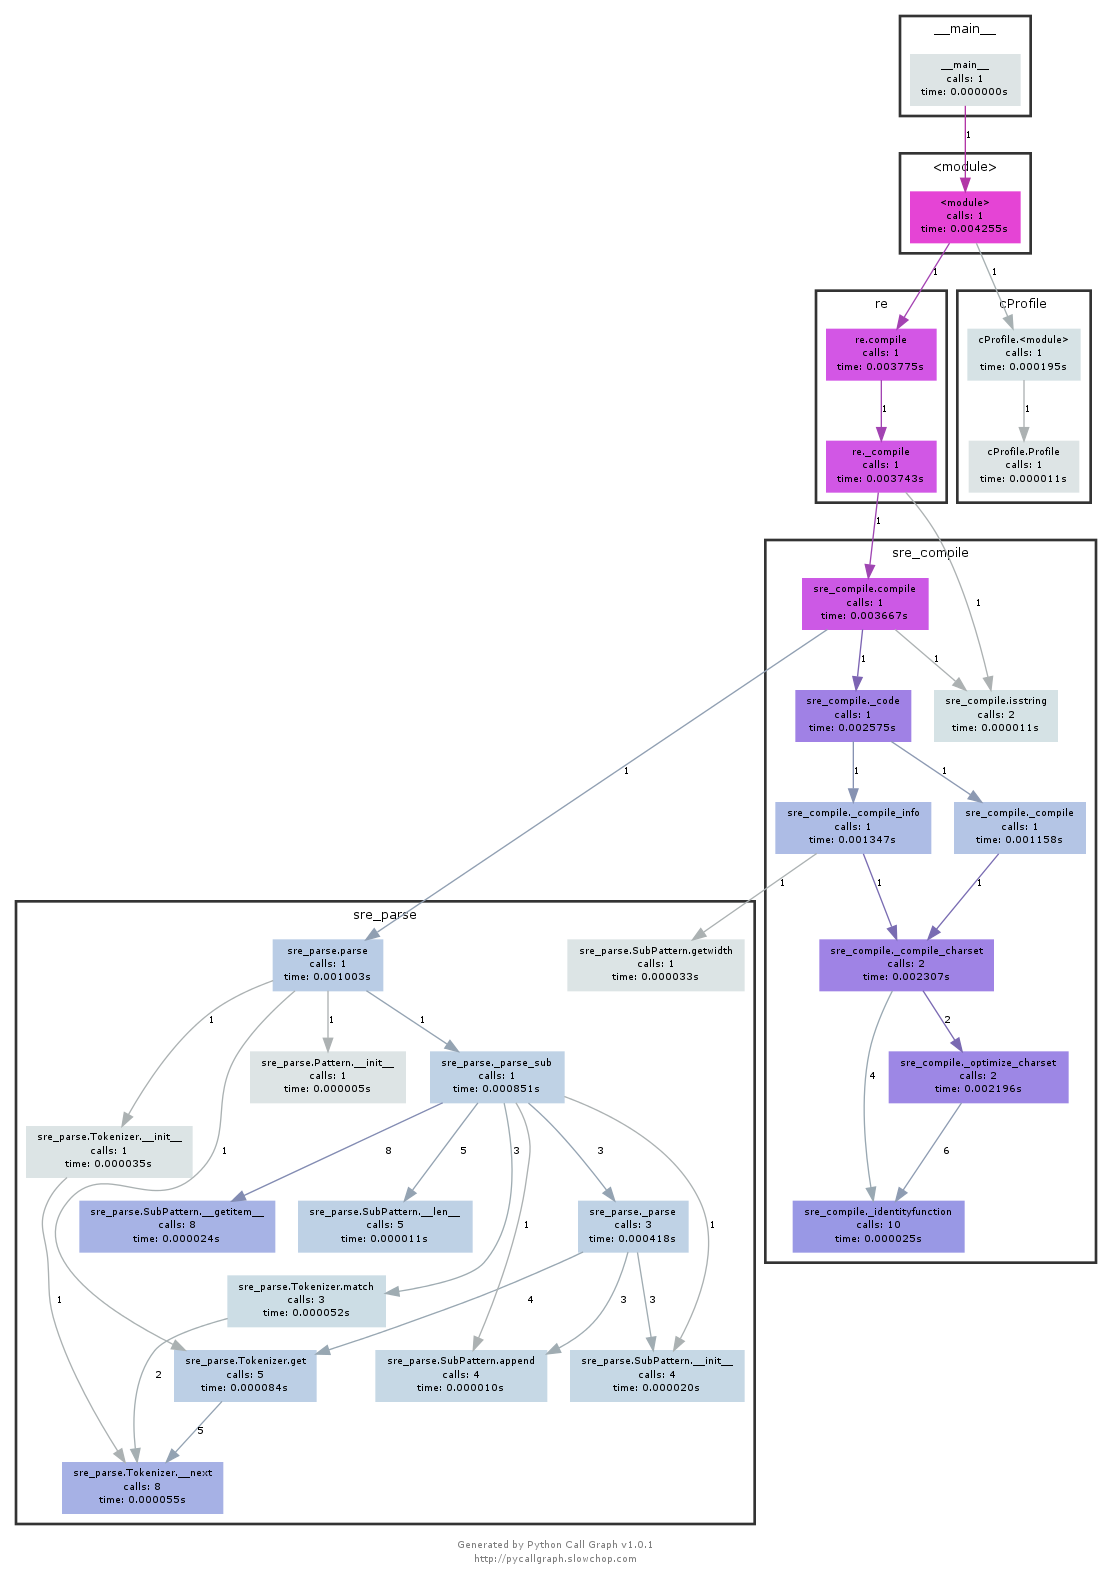
\includegraphics[scale=0.3]{images/re_compile_callgraph.png}
\newpage

%-------------------------------------------------------------------------------
\begin{center}kcachegrid \& pyprof2calltree\end{center}
\begin{verbatim}
$ python -m cProfile -o profile_data.pyprof re_compile.py
$ pyprof2calltree -i profile_data.pyprof -k
\end{verbatim}

\begin{center}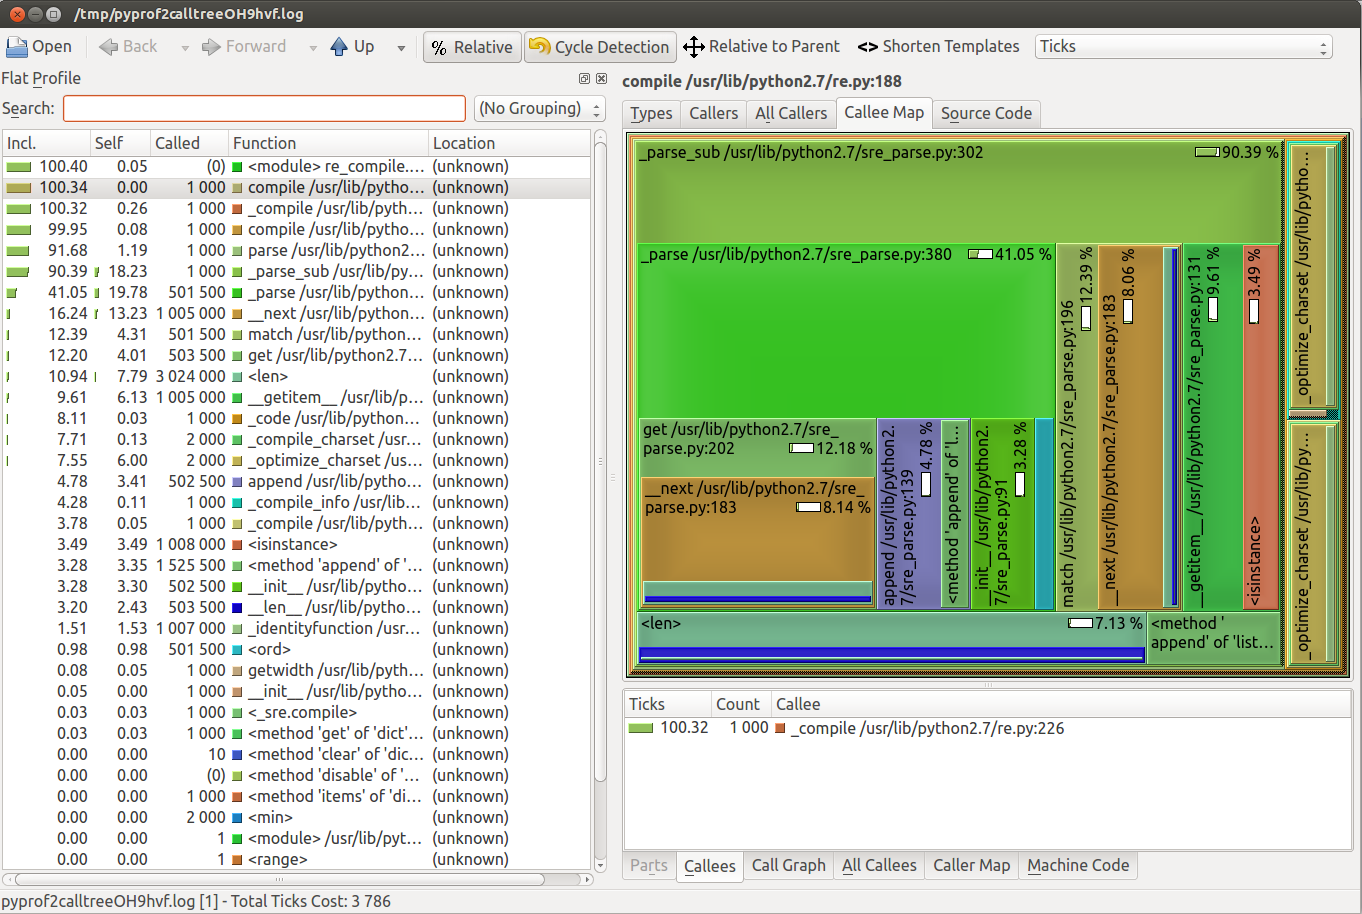
\includegraphics[scale=0.35]{images/kcachegrind.png}\end{center}
\newpage

%-------------------------------------------------------------------------------
\begin{center} runsnakerun \end{center}
\begin{center}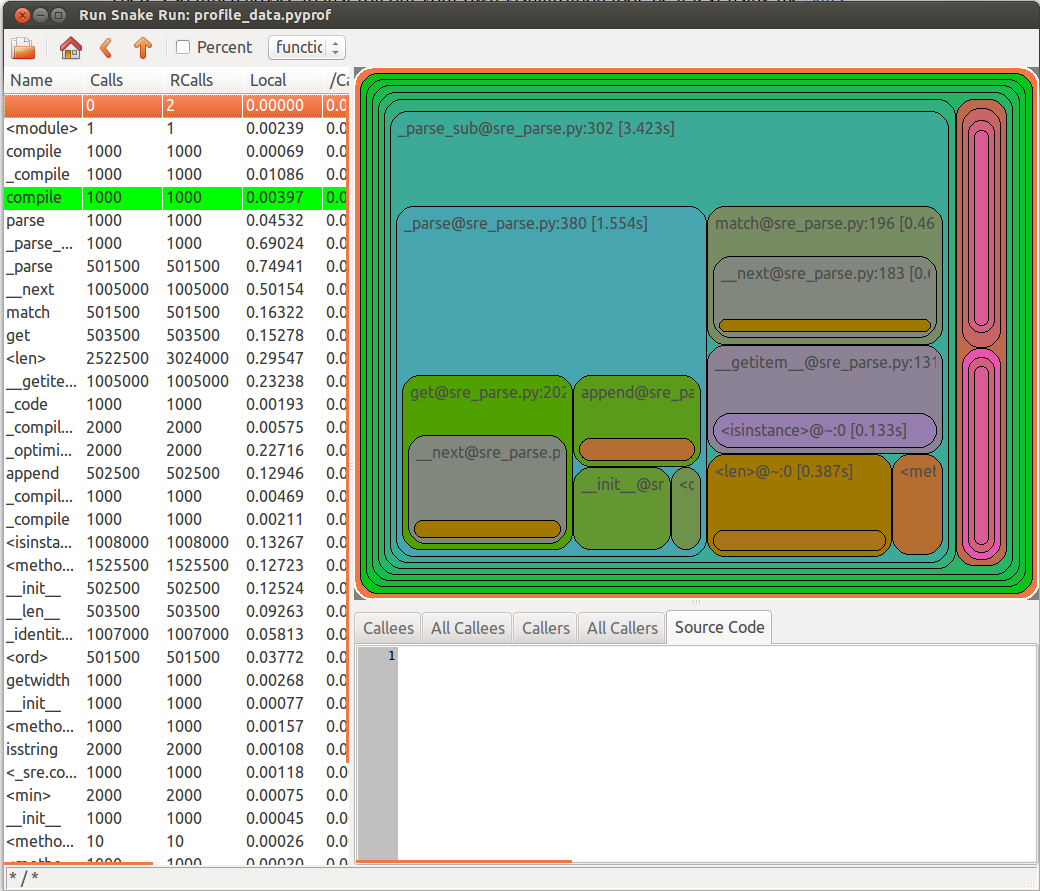
\includegraphics[scale=0.45]{images/runsnake.png}\end{center}
\newpage
%-------------------------------------------------------------------------------
\begin{center} line\_profiler \end{center}
\begin{verbatim}
$ sudo pip install line_profiler
$ kernprof.py -l -v queen_problem.py 12
\end{verbatim}

\begin{lstlisting}
@profile
def hit_to(pos, sz):
    x, y = pos
    cells = [pos]
    for dx in (0, 1, -1):
        for dy in (0, 1, -1):
            if dx == 0 and dy == 0:
                continue

            for i in range(sz):
                nx, ny = x + i * dx, y + i * dy
                if nx < 0 or nx > sz - 1 or ny > sz - 1 or ny < 0:
                    break
                cells.append((nx, ny))
    return cells
\end{lstlisting}
\newpage
%-------------------------------------------------------------------------------
\begin{center} line\_profiler \end{center}
\large
\begin{verbatim}
....
#    Hits    Time PerHit %Time Line Contents
============================================
1                              @profile
2                              def hit_to(pos, sz):
3   81173   34051    0.4   0.4     x, y = pos
4   81173   36006    0.4   0.4     cells = [pos]
5  324692  145524    0.4   1.6     for dx in (0, 1, -1):
6  974076  418874    0.4   4.7         for dy in (0, 1, -1):
7  730557  307418    0.4   3.4             if dx == 0 and dy == 0:
8   81173   31691    0.4   0.4                 continue
9                              
0 4165869 1771034    0.4  19.7             for i in range(sz):
1 4138314 2069723    0.5  23.0                 nx, ny = x + i * dx, y + i * dy
2 4138314 2164515    0.5  24.0                 if nx < 0 or nx > sz - 1 \
                                                   or ny > sz - 1 or ny < 0:
3  621829  293094    0.5   3.3                     break
4 3516485 1699301    0.5  18.9                 cells.append((nx, ny))
5   81173   30539    0.4   0.3     return cells
\end{verbatim}
\LARGE
\newpage

%-------------------------------------------------------------------------------
\begin{center} Профилирование потребления памяти \end{center}
\begin{lstlisting}
sys.getsizeof(1) == 24
sys.getsizeof("1213") == 41
sys.getsizeof([]) == 72
sys.getsizeof([1]) == 80
sys.getsizeof([1, 2]) == 88
sys.getsizeof({1, 2}) == 232
gc.get_referents({1,2,3}) == [1,2,3]
\end{lstlisting}
\newpage

%-------------------------------------------------------------------------------
\begin{center} memory\_profiler \end{center}
\Large
\begin{verbatim}
$ pip install -U memory_profiler
$ python -m memory_profiler example.py
Line #    Mem usage  Increment   Line Contents
==============================================
     3                           @profile
     4      5.97 MB    0.00 MB   def my_func():
     5     13.61 MB    7.64 MB       a = [1] * (10 ** 6)
     6    166.20 MB  152.59 MB       b = [2] * (2 * 10 ** 7)
     7     13.61 MB -152.59 MB       del b
     8     13.61 MB    0.00 MB       return a
\end{verbatim}
\LARGE
\newpage

%-------------------------------------------------------------------------------
\begin{center} Что еще \end{center}
\begin{itemize}
    \item \href{https://bitbucket.org/sumerc/yappi/}{yappi - performance}
    \item \href{http://guppy-pe.sourceforge.net/}{Guppy-PE}
    \item \href{http://mg.pov.lt/objgraph/}{objgraph - memory, obj visualization}
    \item \href{http://pysizer.8325.org/}{PySizer - memory}
    \item resource, psutil
    \item perf, oprofile, sar. perf top
\end{itemize}
\newpage

%-------------------------------------------------------------------------------
\begin{center} ipython \end{center}
\begin{verbatim}
%timeit a + b
%prun some_func
%load_ext memory_profiler
%load_ext line_profiler
%mprun
%lprun
\end{verbatim}
\newpage 

%-------------------------------------------------------------------------------
\begin{center} Оптимизация \end{center}
Скорость исполнения ~O(количество питон инструкций)
\begin{lstlisting}
import dis

def mul2(x):
    return (x + b) << 1
dis.dis(mul2)
\end{lstlisting}

\begin{verbatim}
  0 LOAD_FAST                0 (x)
  3 LOAD_GLOBAL              0 (b)
  6 BINARY_ADD          
  7 LOAD_CONST               1 (1)
 10 BINARY_LSHIFT       
 11 RETURN_VALUE   
\end{verbatim}
\newpage 

%-------------------------------------------------------------------------------
\begin{center} Низкоуровневая оптимизация \end{center}
\begin{itemize}
    \item Локальные переменные быстрее глобальных
    \item Взятие атрибута - дорогая операция
    \item Кешируйте, где можно
    \item Ищите подходящие встроенные методы
    \item cython/C++
    \item \href{https://wiki.python.org/moin/PythonSpeed/PerformanceTips}{PerformanceTips}
    \item \href{http://stackoverflow.com/questions/7165465/optimizing-python-code}{optimizing-python-code}
\end{itemize}
\newpage 

%-------------------------------------------------------------------------------
\begin{center} Локальные переменные быстрее глобальных \end{center}
\begin{verbatim}
def c1(data):                              
    len(data); len(data); len(data); len(data); len(data)

%timeit c1(data)
1000000 loops, best of 3: 238 ns per loop

def c2(data):                              
    ln=len;ln(data); ln(data); ln(data); ln(data); ln(data)

%timeit c2(data)
10000000 loops, best of 3: 196 ns per loop
\end{verbatim}
\newpage 

%-------------------------------------------------------------------------------
\begin{center} Доступ к атрибуту - дорогой \end{center}
\begin{verbatim}
def r1():
    res = []
    for i in xrange(1000):
        res.append(i)

def r2():
    res = []
    a = res.append
    for i in xrange(1000):
        a(i)

%timeit r1()
10000 loops, best of 3: 56.9 µs per loop

%timeit r2()
10000 loops, best of 3: 33.1 µs per loop
\end{verbatim}
\newpage 

%-------------------------------------------------------------------------------
\begin{center}Кешируйте, где можно\end{center}
Шахматы
\newpage 

%-------------------------------------------------------------------------------
\begin{center}Ищите подходящие встроенные методы\end{center}
\begin{itemize}
    \item dict.setdefault
    \item dict.get
    \item sort
    \item heapq
    \item set operations
\end{itemize}
\newpage 
%-------------------------------------------------------------------------------

\end{document}



% ipython embedding
% rpyc
% remote debugging
% introspection
